\documentclass[a4paper]{article}

\usepackage{amsmath}
\usepackage{amssymb}
\usepackage{cancel}
\usepackage{stellar}
\usepackage{parskip}
\usepackage{fullpage}
\usepackage{tikz}
\usepackage{wrapfig}
\usepackage{xfrac}
\usepackage{witharrows}
\usepackage{mathrsfs}

\WithArrowsOptions{displaystyle}

\usetikzlibrary{calc}
\usetikzlibrary{decorations.markings}
\usetikzlibrary{cd}
\usetikzlibrary{positioning}
\usetikzlibrary{angles}

% Cancel color
\renewcommand{\CancelColor}{\color{red}}

\title{Differential geometry}
\author{Paolo Bettelini}
\date{}

\begin{document}

\maketitle

\section{Esercizi}

\begin{snippetexercise}{1 - Proprietà del baricentro di un triangolo}
    \begin{wrapfigure}{r}{6.25cm}
        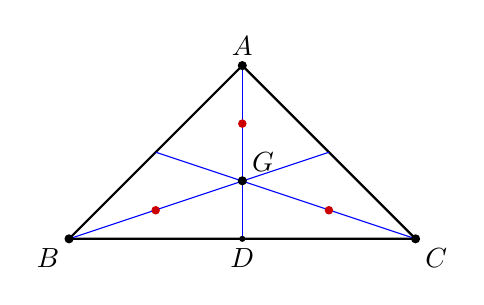
\begin{tikzpicture}[scale=1.1]
            \coordinate (A) at (0,2);
            \coordinate (B) at (-2,0);
            \coordinate (C) at (2,0);
            \coordinate (D) at (0,0);
            \coordinate (E) at (1,1);
            \coordinate (F) at (-1,1);
            \coordinate (G) at (0,0.67);

            \coordinate (H) at (0,1.33);
            \coordinate (I) at (-1,0.33);
            \coordinate (L) at (1,0.33);

            \draw[thick] (A)--(B)--(C)--cycle;
            \draw[blue] (A)--(D);
            \draw[blue] (B)--(E);
            \draw[blue] (C)--(F);

            \fill (A) circle (1.5pt) node[above] {\(A\)};
            \fill (B) circle (1.5pt) node[below left] {\(B\)};
            \fill (C) circle (1.5pt) node[below right] {\(C\)};
            \fill (G) circle (1.5pt) node[above right] {\(G\)};
            \fill (D) circle (1pt) node[below] {\(D\)};

            \fill[red!80!black] (H) circle (1.4pt);
            \fill[red!80!black] (I) circle (1.4pt);
            \fill[red!80!black] (L) circle (1.4pt);
        \end{tikzpicture}
        \vspace{-1.25cm}
    \end{wrapfigure}
    Sia \(ABC\) un triangolo. Dimostrare che le tre mediane si
    incontrano in un unico punto \(G\), detto \emph{baricentro}, e che
    \(G\) divide ciascuna mediana in due parti, una doppia dell'altra.
    Più precisamente, se \(D\) è il punto medio di \(BC\), allora
    \(AG = 2GD\). \wrapfill
\end{snippetexercise}

\begin{snippetsolution}{1 - Proprietà del baricentro di un triangolo}
    Scegliamo un'origine e identifichiamo i punti \(A,B,C\) con i loro vettori posizione. Poniamo
    \[
        G = \frac13(A+B+C).
    \]
    Sia \(D\) il punto medio di \(BC\), cioè
    \[
        D = \frac12(B+C).
    \]
    Allora
    \begin{align*}
        G &= \frac13 A + \frac13 B + \frac13 C \\
          &= \frac13 A + \frac23 \left(\frac12B+\frac12C\right) \\
          &= \frac13 A + \frac23 D.
    \end{align*}
    Quindi \(G\) appartiene alla retta \(AD\), e più precisamente è il punto della mediana \(AD\) corrispondente al parametro \(t=\frac23\):
    \[
        G = \left(1-\frac23\right)A+\frac23D.
    \]
    Ne segue che
    \[
        AG = \frac23AD,
        \qquad
        GD = \frac13AD,
    \]
    e quindi
    \[
        AG = 2GD.
    \]
    Se ora \(E\) è il punto medio di \(AC\) e \(F\) è il punto medio di \(AB\), analogamente si ha
    \[
        G = \frac13B+\frac23E,
        \qquad
        G = \frac13C+\frac23F.
    \]
    Dunque \(G\) appartiene anche alle mediane \(BE\) e \(CF\). Le tre mediane passano quindi tutte per \(G\). Inoltre, poiché due mediane distinte di un triangolo non degenere non sono parallele, esse si incontrano in un unico punto; pertanto il punto comune alle tre mediane è unico.
\end{snippetsolution}

\begin{snippetexercise}{2 - Problema del biliardo I}
    \begin{wrapfigure}{r}{7.25cm}
        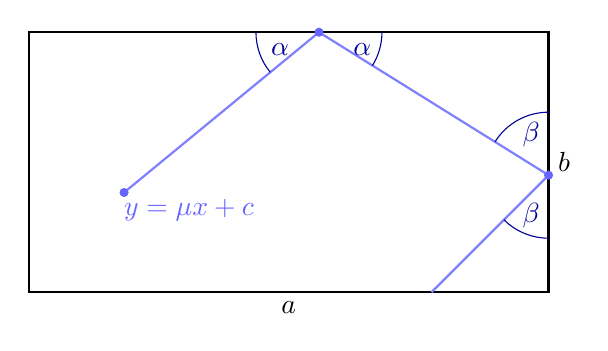
\begin{tikzpicture}[scale=1.1]
            \coordinate (A) at (0,0);
            \coordinate (B) at (6,0);
            \coordinate (C) at (6,3);
            \coordinate (D) at (0,3);

            \coordinate (P) at (1.1,1.15);
            \coordinate (T) at (3.35,3);
            \coordinate (R) at (6,1.35);
            \coordinate (Q) at (4.65,0);

            \coordinate (TL) at (2.5,3);
            \coordinate (TR) at (4.2,3);
            \coordinate (RU) at (6,2.2);
            \coordinate (RD) at (6,0.5);

            \draw[thick] (A)--(B)--(C)--(D)--cycle;
            \draw[blue!50, thick] (P)--(T)--(R)--(Q);

            \fill[blue!60] (P) circle (1.5pt);
            \fill[blue!60] (T) circle (1.5pt);
            \fill[blue!60] (R) circle (1.5pt);

            \node[below] at (3,0) {\(a\)};
            \node[right] at (6,1.5) {\(b\)};

            \node[blue!60] at (1.85,0.95) {\(y=\mu x+c\)};

            \pic[draw=blue!60!black, angle radius=8mm, angle eccentricity=1.25] {angle = TL--T--P};
            \pic[draw=blue!60!black, angle radius=8mm, angle eccentricity=1.25] {angle = R--T--TR};

            \pic[draw=blue!60!black, angle radius=8mm, angle eccentricity=1.25] {angle = RU--R--T};
            \pic[draw=blue!60!black, angle radius=8mm, angle eccentricity=1.25] {angle = Q--R--RD};

            \node[blue!60!black] at (2.9,2.8) {\(\alpha\)};
            \node[blue!60!black] at (3.85,2.8) {\(\alpha\)};
            \node[blue!60!black] at (5.8,1.82) {\(\beta\)};
            \node[blue!60!black] at (5.8,0.88) {\(\beta\)};
        \end{tikzpicture}
        \vspace{-1.25cm}
    \end{wrapfigure}
    Si consideri un biliardo rettangolare senza attriti, con lati di
    lunghezze \(a\) e \(b\). Supponiamo che il coefficiente angolare
    \(\mu\) della direzione del tiro sia commensurabile con
    \(\frac{b}{a}\), cioè che esistano \(m,n\in\naturalnumbers\) tali che
    \[
        \mu = \frac{mb}{na}.
    \]
    Dimostrare che la traiettoria è periodica. \wrapfill
\end{snippetexercise}

\begin{snippetsolution}{2 - Problema del biliardo I}
    Consideriamo il biliardo sviluppato per riflessione. Invece di riflettere la traiettoria sui lati del rettangolo, riflettiamo il rettangolo stesso: nel piano così ottenuto la traiettoria diventa una retta.
    Sia \((x_0,y_0)\) il punto iniziale. Poiché
    \[
        \mu=\frac{mb}{na},
    \]
    possiamo parametrizzare la retta nel piano sviluppato come
    \[
        x(t)=nat+x_0,
        \qquad
        y(t)=mbt+y_0.
    \]
    Infatti il suo coefficiente angolare è
    \[
        \frac{mb}{na}=\mu.
    \]
    Nel piano sviluppato due punti danno lo stesso punto del biliardo con la stessa direzione quando differiscono di un multiplo di \(2a\) nella coordinata \(x\) e di un multiplo di \(2b\) nella coordinata \(y\). Consideriamo allora il tempo \(t=2\). Si ha
    \begin{align*}
        x(2)&=2na+x_0=x_0+n(2a),\\
        y(2)&=2mb+y_0=y_0+m(2b).
    \end{align*}
    Dunque, nel piano sviluppato, il punto \(c(2)\) è equivalente al punto iniziale \(c(0)=(x_0,y_0)\) rispetto ai periodi \(2a\) e \(2b\). Ripiegando il piano sviluppato sul rettangolo iniziale, la traiettoria torna quindi nello stesso punto del biliardo e con la stessa direzione.
    Pertanto, dopo un numero finito di riflessioni, la traiettoria si ripete: la traiettoria è periodica.
\end{snippetsolution}

\begin{snippetexercise}{3 - Problema del biliardo II}
    Con la stessa notazione dell'esercizio precedente, dimostrare che
    se \(\mu\) non è commensurabile con \(\frac{b}{a}\), cioè
    \[
        \frac{\mu}{b/a}\notin\rationalnumbers,
    \]
    allora la traiettoria è densa nel biliardo.
\end{snippetexercise}

\begin{snippetsolution}{3 - Problema del biliardo II}
    Consideriamo ancora il biliardo sviluppato per riflessione. Nel piano sviluppato la traiettoria diventa la retta
    \[
        y-y_0=\mu(x-x_0).
    \]
    Poniamo
    \[
        \alpha=\frac{\mu a}{b}.
    \]
    Per ipotesi \(\alpha\notin\rationalnumbers\). Passiamo ora al quoziente rispetto al reticolo di periodi \(2a\) e \(2b\), cioè identifichiamo i punti che differiscono di un vettore di \(2a\integernumbers\times 2b\integernumbers\). In coordinate normalizzate
    \[
        u=\frac{x}{2a},
        \qquad
        v=\frac{y}{2b},
    \]
    la retta sviluppata diventa, modulo \(\integernumbers^2\),
    \[
        (u(t),v(t))=(u_0,v_0)+t(1,\alpha).
    \]
    Poiché \(\alpha\notin\rationalnumbers\), per il risultato sulle orbite modulo un reticolo, l'orbita
    \[
        \{(u_0+t,v_0+\alpha t)\mod \integernumbers^2\mid t\in\realnumbers\}
    \]
    è densa nel toro \(\realnumbers^2/\integernumbers^2\).
    Ripiegare il piano sviluppato sul rettangolo iniziale significa applicare la mappa continua che identifica ogni copia riflessa del rettangolo con il biliardo \(S=[0,a]\times[0,b]\). Questa mappa manda il toro con periodi \(2a\) e \(2b\) sul rettangolo \(S\), e la traiettoria del biliardo è precisamente l'immagine dell'orbita precedente.
    L'immagine continua di un insieme denso è densa nell'immagine. Quindi la traiettoria ripiegata è densa in \(S\). Pertanto, se \(\mu\) non è commensurabile con \(\frac ba\), la traiettoria è densa nel biliardo.
\end{snippetsolution}

\begin{snippetexercise}{4 - Studio del nodo semplice}
    \begin{wrapfigure}{r}{6.25cm}
        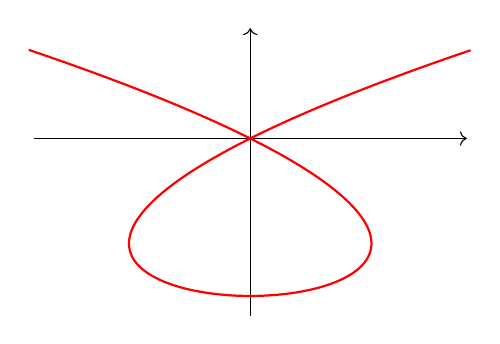
\begin{tikzpicture}[scale=0.5]
            \draw[->] (-5.5,0) -- (5.5,0);
            \draw[->] (0,-4.5) -- (0,2.8);

            \draw[red, thick, smooth, samples=200, domain=-2.5:2.5, variable=\t]
                plot ({\t*\t*\t - 4*\t}, {\t*\t - 4});
        \end{tikzpicture}
        \vspace{-1cm}
    \end{wrapfigure}
    Studiare la curva
    \[
        \sigma\colon\realnumbers\to\realnumbers^2,
        \qquad
        \sigma(t)=\left(t^3-t,t^2-t\right).
    \]
    In particolare, determinare se la curva è regolare, individuare
    eventuali autointersezioni e descrivere il comportamento locale nel
    punto doppio. \wrapfill
\end{snippetexercise}

\begin{snippetsolution}{4 - Studio del nodo semplice}
    Calcoliamo innanzitutto la derivata:
    \[
        \sigma'(t)=\left(3t^2-1,2t-1\right).
    \]
    La curva non è regolare solo se \(\sigma'(t)=0\), cioè se
    \[
        \begin{cases}
            3t^2-1=0,\\
            2t-1=0.
        \end{cases}
    \]
    Dalla seconda equazione si ha \(t=\frac12\), ma allora
    \[
        3t^2-1=3\cdot\frac14-1=-\frac14\neq 0.
    \]
    Quindi non esiste alcun \(t\in\realnumbers\) tale che \(\sigma'(t)=0\), e la curva è regolare.
    Cerchiamo ora le autointersezioni. Siano \(t_1<t_2\) tali che \(\sigma(t_1)=\sigma(t_2)\). Allora
    \begin{align*}
        \sigma(t_1)=\sigma(t_2)
        \iff
        \begin{cases}
            t_1^3-t_1=t_2^3-t_2,\\
            t_1^2-t_1=t_2^2-t_2.
        \end{cases}
    \end{align*}
    Poiché \(t_1\neq t_2\), possiamo fattorizzare e dividere per \(t_1-t_2\). Otteniamo
    \[
        \begin{cases}
            t_1^2+t_1t_2+t_2^2-1=0,\\
            t_1+t_2-1=0.
        \end{cases}
    \]
    Dalla seconda equazione \(t_1+t_2=1\). Allora
    \[
        t_1^2+t_1t_2+t_2^2=(t_1+t_2)^2-t_1t_2=1-t_1t_2.
    \]
    Sostituendo nella prima equazione si ottiene
    \[
        1-t_1t_2-1=0,
    \]
    cioè \(t_1t_2=0\). Dunque \(t_1,t_2\) hanno somma \(1\) e prodotto \(0\), quindi
    \[
        \{t_1,t_2\}=\{0,1\}.
    \]
    Infatti
    \[
        \sigma(0)=(0,0),
        \qquad
        \sigma(1)=(0,0).
    \]
    L'unica autointersezione è quindi l'origine.
    Studiamo infine il comportamento locale nel punto doppio. I due rami che passano per l'origine corrispondono ai parametri \(t=0\) e \(t=1\). Le rispettive direzioni tangenti sono
    \[
        \sigma'(0)=(-1,-1),
        \qquad
        \sigma'(1)=(2,1).
    \]
    Quindi le due tangenti nel punto doppio sono
    \[
        y=x,
        \qquad
        y=\frac12x.
    \]
    Poiché queste rette sono distinte, i due rami si intersecano trasversalmente. Dunque l'origine è un punto doppio ordinario, cioè un nodo semplice.
\end{snippetsolution}

\pagebreak

\begin{snippetexercise}{5 - Folium di Cartesio}
    \begin{wrapfigure}{r}{6.25cm}
        \begin{tikzpicture}[scale=0.75]
            \clip (-4,-4) rectangle (4,4);
            \draw[->] (-4,0) -- (4,0);
            \draw[->] (0,-4) -- (0,4);
            \draw[dashed] (-4,3) -- (3,-4);

            \draw[red, thick, smooth, samples=300, domain=0:25, variable=\t]
                plot ({3*\t/(1+\t*\t*\t)}, {3*\t*\t/(1+\t*\t*\t)});

            \draw[red, thick, smooth, samples=300, domain=-12:-1.05, variable=\t]
                plot ({3*\t/(1+\t*\t*\t)}, {3*\t*\t/(1+\t*\t*\t)});

            \draw[red, thick, smooth, samples=300, domain=-0.95:-0.03, variable=\t]
                plot ({3*\t/(1+\t*\t*\t)}, {3*\t*\t/(1+\t*\t*\t)});
        \end{tikzpicture}
        \vspace{-1.25cm}
    \end{wrapfigure}
    Studiare il folium di Cartesio parametrizzato da
    \[
        \sigma\colon(-1,+\infty)\to\realnumbers^2,
        \qquad
        \sigma(t)=
        \left(
            \frac{3t}{1+t^3},
            \frac{3t^2}{1+t^3}
        \right).
    \]
    Dimostrare che la curva è regolare e iniettiva, e spiegare in che
    senso essa si autointerseca all'infinito. \wrapfill
\end{snippetexercise}

\begin{snippetsolution}{5 - Folium di Cartesio}
    Calcoliamo innanzitutto la derivata:
    \begin{align*}
        \sigma'(t)
        &=
        \left(
            \frac{3(1+t^3)-9t^3}{(1+t^3)^2},
            \frac{6t(1+t^3)-9t^4}{(1+t^3)^2}
        \right)\\
        &=
        \left(
            \frac{3-6t^3}{(1+t^3)^2},
            \frac{6t-3t^4}{(1+t^3)^2}
        \right).
    \end{align*}
    Quindi \(\sigma'(t)=(0,0)\) se e solo se
    \[
        \begin{cases}
            3-6t^3=0,\\
            6t-3t^4=0.
        \end{cases}
    \]
    La prima equazione dà \(t^3=\frac12\), mentre la seconda dà
    \[
        3t(2-t^3)=0,
    \]
    cioè \(t=0\) oppure \(t^3=2\). Le due equazioni non possono quindi essere verificate simultaneamente. Dunque \(\sigma\) è regolare su \((-1,+\infty)\).
    Mostriamo ora che \(\sigma\) è iniettiva. Se \(t\neq 0\), allora la prima coordinata è non nulla e si può recuperare il parametro dal punto della curva:
    \[
        \frac{y(t)}{x(t)}
        =
        \frac{\frac{3t^2}{1+t^3}}{\frac{3t}{1+t^3}}
        =
        t.
    \]
    Se invece \(x(t)=0\), allora necessariamente \(t=0\), e infatti
    \[
        \sigma(0)=(0,0).
    \]
    Quindi due parametri distinti non possono avere la stessa immagine, e \(\sigma\) è iniettiva.
    Studiamo infine il comportamento agli estremi del dominio. Per \(t\to -1^+\), le coordinate divergono e si ha
    \[
        x(t)+y(t)+1
        =
        \frac{3t+3t^2}{1+t^3}+1
        =
        \frac{3t}{1-t+t^2}+1
        =
        \frac{(t+1)^2}{1-t+t^2}
        \longrightarrow 0.
    \]
    Quindi la curva ha asintoto
    \[
        x+y+1=0.
    \]
    Per \(t\to+\infty\), invece,
    \[
        \lim_{t\to+\infty}\sigma(t)=(0,0)=\sigma(0).
    \]
    Dunque la curva non si autointerseca per valori finiti del parametro, perché è iniettiva, ma torna all'origine quando il parametro tende a \(+\infty\). In questo senso l'autointersezione avviene all'infinito del parametro.
    Più precisamente, se si compatta il dominio aggiungendo il punto \(+\infty\), allora la mappa estesa soddisfa
    \[
        \sigma(+\infty)=\sigma(0)=(0,0).
    \]
    Il ramo corrispondente a \(t=0\) ha tangente
    \[
        \sigma'(0)=(3,0),
    \]
    mentre il ramo corrispondente a \(t=+\infty\), ponendo \(s=\frac1t\), è
    \[
        \sigma\left(\frac1s\right)
        =
        \left(
            \frac{3s^2}{1+s^3},
            \frac{3s}{1+s^3}
        \right),
    \]
    e ha tangente in \(s=0\)
    \[
        \left(\sigma\left(\frac1s\right)\right)'_{s=0}=(0,3).
    \]
    I due rami hanno quindi tangenti distinte, e l'origine diventa un nodo se si considera anche il punto \(t=+\infty\).
\end{snippetsolution}

\begin{snippetexercise}{6 - Metrica su sottoinsiemi connessi da archi rettificabili}
    Sia \(X\subseteq\realnumbers^m\) con la seguente proprietà: per
    ogni \(P,Q\in X\) esiste una curva
    \[
        \sigma\colon[a,b]\to X
    \]
    di classe \(C^1\) a tratti tale che
    \[
        \sigma(a)=P,
        \qquad
        \sigma(b)=Q.
    \]
    Definiamo
    \[
        d_X(P,Q)=\inf\left\{L(\sigma)\mid \sigma \text{ curva come sopra
        che congiunge } P \text{ e } Q\right\}.
    \]
    Dimostrare che \(d_X\) è una metrica su \(X\).
\end{snippetexercise}

\begin{snippetsolution}{6 - Metrica su sottoinsiemi connessi da archi rettificabili}
    Per ipotesi, per ogni \(P,Q\in X\) esiste almeno una curva \(C^1\) a tratti che congiunge \(P\) a \(Q\). Inoltre ogni curva \(C^1\) a tratti ha lunghezza finita. Dunque \(d_X(P,Q)\) è ben definita e finita.
    La non negatività è immediata, poiché
    \[
        L(\sigma)\geq 0
    \]
    per ogni curva \(\sigma\). Quindi
    \[
        d_X(P,Q)\geq 0.
    \]
    Inoltre, per la proposizione sulla lunghezza delle curve \(C^1\) a tratti, se \(\sigma\) congiunge \(P\) a \(Q\), allora
    \[
        L(\sigma)\geq \left\|P-Q\right\|.
    \]
    Passando all'inf su tutte le curve ammissibili otteniamo
    \[
        d_X(P,Q)\geq \left\|P-Q\right\|.
    \]
    Quindi, se \(d_X(P,Q)=0\), allora \(\left\|P-Q\right\|=0\), e dunque \(P=Q\). Viceversa, se \(P=Q\), possiamo considerare la curva costante \(\sigma(t)=P\), che ha lunghezza nulla. Pertanto
    \[
        d_X(P,P)=0.
    \]
    Dimostriamo ora la simmetria. Se \(\sigma\colon[a,b]\to X\) congiunge \(P\) a \(Q\), allora la curva percorsa al contrario
    \[
        \widetilde{\sigma}(t)=\sigma(a+b-t)
    \]
    congiunge \(Q\) a \(P\) e ha la stessa lunghezza:
    \[
        L(\widetilde{\sigma})=L(\sigma).
    \]
    Passando all'inf sulle curve ammissibili si ottiene
    \[
        d_X(P,Q)=d_X(Q,P).
    \]
    Infine dimostriamo la disuguaglianza triangolare. Siano \(P,Q,R\in X\). Se \(\sigma_1\) congiunge \(P\) a \(Q\) e \(\sigma_2\) congiunge \(Q\) a \(R\), allora la concatenazione \(\sigma_1*\sigma_2\) congiunge \(P\) a \(R\) ed è ancora \(C^1\) a tratti. Inoltre
    \[
        L(\sigma_1*\sigma_2)=L(\sigma_1)+L(\sigma_2).
    \]
    Quindi
    \[
        d_X(P,R)\leq L(\sigma_1*\sigma_2)=L(\sigma_1)+L(\sigma_2).
    \]
    Passando all'inf prima su \(\sigma_1\) e poi su \(\sigma_2\), otteniamo
    \[
        d_X(P,R)\leq d_X(P,Q)+d_X(Q,R).
    \]
    Dunque \(d_X\) soddisfa tutti gli assiomi di una metrica su \(X\).
\end{snippetsolution}

\begin{snippetexercise}{7 - Distanze su cono circolare}
    \begin{wrapfigure}{r}{4.6cm}
        \centering
        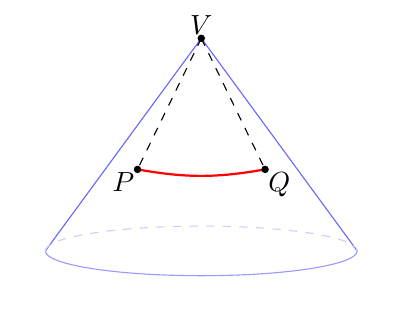
\begin{tikzpicture}[scale=0.9]
            \useasboundingbox (-2.45,-0.45) rectangle (2.45,3.15);

            \coordinate (V) at (0,3);
            \coordinate (P) at (-0.9,1.15);
            \coordinate (Q) at (0.9,1.15);

            \draw[blue!60] (V)--(-2.2,0);
            \draw[blue!60] (V)--(2.2,0);
            \draw[blue!40] (-2.2,0) arc (180:360:2.2 and 0.35);
            \draw[blue!20,dashed] (-2.2,0) arc (180:0:2.2 and 0.35);

            \draw[dashed] (V)--(P);
            \draw[dashed] (V)--(Q);
            \draw[red,thick] (P) to[out=-10,in=190] (Q);

            \fill (V) circle (1.5pt) node[above,inner sep=1pt] {\(V\)};
            \fill (P) circle (1.5pt) node[below left,inner sep=1pt] {\(P\)};
            \fill (Q) circle (1.5pt) node[below right,inner sep=1pt] {\(Q\)};
        \end{tikzpicture}
    \end{wrapfigure}
    Sia \(X\) un cono circolare, definito come la superficie di
    rotazione della retta \(\ell\subseteq\realnumbers^2_{yz}\) intorno
    all'asse \(z\). Denotiamo con \(\theta\) l'angolo tra \(\ell\) e
    l'asse \(z\).
    Siano \(P,Q\in X\) due punti alla stessa altezza, cioè
    \(z(P)=z(Q)\). Si considerino:
    \[
        c = \text{arco di circonferenza del parallelo che congiunge } P
        \text{ e } Q,
    \]
    e
    \[
        \tau=[P,V]\union[Q,V],
    \]
    dove \(V\) è il vertice del cono.
    Trovare il valore limite di \(\theta\) che separa i casi in cui la
    distanza intrinseca \(d_X(P,Q)\) è realizzata dall'arco \(c\) da
    quelli in cui è realizzata dal cammino spezzato \(\tau\). \wrapfill
\end{snippetexercise}

\begin{snippetsolution}{7 - Distanze su cono circolare}
    Sviluppiamo il cono sul piano tagliandolo lungo una generatrice. Le generatrici del cono diventano raggi di un settore circolare. Se
    \[
        \ell=\left\|P-V\right\|=\left\|Q-V\right\|,
    \]
    allora il raggio del parallelo alla quota di \(P\) e \(Q\) è
    \[
        r=\ell\sin\theta.
    \]
    Supponiamo che \(P\) e \(Q\) siano opposti sul parallelo. Allora l'arco di parallelo che li congiunge è una semicirconferenza di raggio \(r\), quindi ha lunghezza
    \[
        L(c)=\pi r=\pi\ell\sin\theta.
    \]
    Il cammino spezzato che passa per il vertice ha invece lunghezza
    \[
        L(\tau)=\left\|P-V\right\|+\left\|V-Q\right\|=2\ell.
    \]
    Il valore limite di \(\theta\) si ottiene imponendo l'uguaglianza tra le due lunghezze:
    \begin{align*}
        \pi\ell\sin\theta &= 2\ell,\\
        \pi\sin\theta &= 2,\\
        \sin\theta &= \frac{2}{\pi}.
    \end{align*}
    Dunque
    \[
        \theta_0=\arcsin\left(\frac{2}{\pi}\right).
    \]
    Se \(0<\theta<\theta_0\), allora
    \[
        \pi\ell\sin\theta<2\ell,
    \]
    quindi la distanza intrinseca è realizzata dall'arco di parallelo \(c\). Se invece \(\theta>\theta_0\), allora
    \[
        \pi\ell\sin\theta>2\ell,
    \]
    quindi è più corto il cammino spezzato \(\tau=[P,V]\union[V,Q]\). Nel caso limite \(\theta=\theta_0\), i due cammini hanno la stessa lunghezza.
\end{snippetsolution}

\begin{snippetexercise}{8 - Spirale logaritmica}
    \begin{wrapfigure}{r}{5.25cm}
        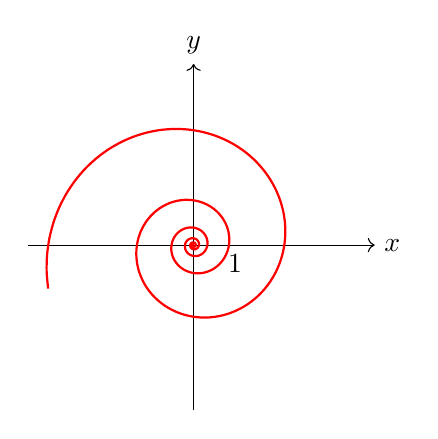
\begin{tikzpicture}[scale=0.5]
            \draw[->] (-4.2,0) -- (4.6,0) node[right] {\(x\)};
            \draw[->] (0,-4.2) -- (0,4.6) node[above] {\(y\)};
            \draw[red, thick, smooth, samples=300, domain=-18:16]
                plot ({0.35*exp(0.15*\x)*cos(\x r)},{0.35*exp(0.15*\x)*sin(\x r)});
            \draw (1.05,0) node[below] {\(1\)};
        \end{tikzpicture}
        \vspace{-1cm}
    \end{wrapfigure}
    Calcolare una parametrizzazione per lunghezza d'arco della
    spirale logaritmica
    \[
        \sigma\colon\realnumbers\to\realnumbers^2,
        \qquad
        \sigma(t)=e^t(\cos t,\sin t).
    \]
    Calcolare inoltre la lunghezza della restrizione
    \[
        \sigma\big|_{(-\infty,0]}.
    \]
    \wrapfill
\end{snippetexercise}

\begin{snippetsolution}{8 - Spirale logaritmica}
    Calcoliamo innanzitutto la derivata:
    \[
        \sigma'(t)=e^t(\cos t,\sin t)+e^t(-\sin t,\cos t)
        =
        e^t(\cos t-\sin t,\sin t+\cos t).
    \]
    Quindi
    \begin{align*}
        \left\|\sigma'(t)\right\|
        &=
        e^t\sqrt{(\cos t-\sin t)^2+(\sin t+\cos t)^2}\\
        &=
        e^t\sqrt{2}
        =
        \sqrt{2}e^t.
    \end{align*}
    Scegliamo come parametro di lunghezza d'arco
    \[
        s(t)=\int_0^t \left\|\sigma'(\tau)\right\|\,d\tau
        =
        \int_0^t \sqrt{2}e^\tau\,d\tau
        =
        \sqrt{2}(e^t-1).
    \]
    Da cui
    \[
        e^t=1+\frac{s}{\sqrt{2}},
        \qquad
        t=\log\left(1+\frac{s}{\sqrt{2}}\right).
    \]
    Il dominio del nuovo parametro è
    \[
        s\in(-\sqrt{2},+\infty).
    \]
    Dunque una parametrizzazione per lunghezza d'arco è
    \[
        \gamma(s)
        =
        \sigma\left(\log\left(1+\frac{s}{\sqrt{2}}\right)\right),
        \qquad s\in(-\sqrt{2},+\infty),
    \]
    cioè
    \[
        \gamma(s)
        =
        \left(1+\frac{s}{\sqrt{2}}\right)
        \left(
            \cos\left(\log\left(1+\frac{s}{\sqrt{2}}\right)\right),
            \sin\left(\log\left(1+\frac{s}{\sqrt{2}}\right)\right)
        \right).
    \]
    Infine,
    \[
        L\left(\sigma\big|_{(-\infty,0]}\right)
        =
        \int_{-\infty}^{0}\sqrt{2}e^t\,dt
        =
        \sqrt{2}.
    \]
\end{snippetsolution}

\begin{snippetexercise}{9 - Elica circolare}
    \begin{wrapfigure}{r}{6.8cm}
        \centering
        \begin{minipage}{0.48\linewidth}
            \centering
            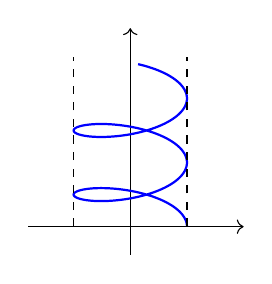
\begin{tikzpicture}[scale=0.72]
                \draw[->] (-1.8,0)--(2,0);
                \draw[->] (0,-0.5)--(0,3.5);
                \draw[blue,thick,domain=0:14,samples=220,smooth,variable=\u]
                    plot ({cos(\u r)},{0.18*\u+0.35*sin(\u r)});
                \draw[dashed] (-1,0)--(-1,3);
                \draw[dashed] (1,0)--(1,3);
            \end{tikzpicture}
        \end{minipage}
        \hfill
        \begin{minipage}{0.48\linewidth}
            \centering
            \begin{tikzpicture}[scale=0.72]
                \draw[->] (0,0) -- (-1.2,-0.8) node[below] {\(x\)};
                \draw[->] (0,0) -- (1.6,0) node[right] {\(y\)};
                \draw[->] (0,0) -- (0,2.8) node[above] {\(z\)};
                \draw[smooth, samples=120, domain=0:6.2]
                    plot ({0.55*cos(\x r)},{0.25*sin(\x r)+0.35*\x});
            \end{tikzpicture}
        \end{minipage}
    \end{wrapfigure}
    Calcolare la funzione curvatura dell'elica circolare
    \[
        \sigma\colon\realnumbers\to\realnumbers^3,
        \qquad
        \sigma(t)=(\cos t,\sin t,at),
    \]
    dove \(a\in\realnumbers\). \wrapfill
\end{snippetexercise}

\begin{snippetsolution}{9 - Elica circolare}
    Calcoliamo le prime derivate:
    \[
        \sigma'(t)=(-\sin t,\cos t,a),
        \qquad
        \sigma''(t)=(-\cos t,-\sin t,0).
    \]
    La velocità ha modulo costante:
    \[
        \left\|\sigma'(t)\right\|
        =
        \sqrt{\sin^2t+\cos^2t+a^2}
        =
        \sqrt{1+a^2}.
    \]
    Poniamo quindi
    \[
        M=\sqrt{1+a^2}.
    \]
    Una parametrizzazione per lunghezza d'arco è
    \[
        \gamma(s)=\sigma\left(\frac{s}{M}\right).
    \]
    Infatti
    \[
        \gamma'(s)=\sigma'\left(\frac{s}{M}\right)\frac1M
    \]
    e dunque
    \[
        \left\|\gamma'(s)\right\|=1.
    \]
    La curvatura è allora
    \[
        k(s)=\left\|\gamma''(s)\right\|.
    \]
    Calcoliamo:
    \[
        \gamma'(s)
        =
        \frac1M
        \left(
            -\sin\frac{s}{M},
            \cos\frac{s}{M},
            a
        \right),
    \]
    quindi
    \[
        \gamma''(s)
        =
        \frac1{M^2}
        \left(
            -\cos\frac{s}{M},
            -\sin\frac{s}{M},
            0
        \right).
    \]
    Pertanto
    \[
        k(s)
        =
        \left\|\gamma''(s)\right\|
        =
        \frac1{M^2}
        =
        \frac1{1+a^2}.
    \]
    La curvatura dell'elica circolare è quindi costante e vale
    \[
        k=\frac1{1+a^2}.
    \]
\end{snippetsolution}

\begin{snippetexercise}{10 - Doppia elica}
    \begin{wrapfigure}{r}{6.2cm}
        \centering
        \begin{minipage}{0.48\linewidth}
            \centering
            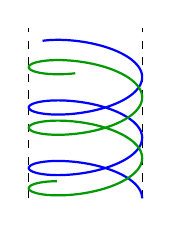
\begin{tikzpicture}[scale=0.72]
                \draw[dashed] (-1,0)--(-1,3);
                \draw[dashed] (1,0)--(1,3);

                \draw[blue,thick,domain=0:15,samples=220,smooth,variable=\u]
                    plot ({cos(\u r)},{0.17*\u+0.35*sin(\u r)});
                \draw[green!60!black,thick,domain=0:15,samples=220,smooth,variable=\u]
                    plot ({cos((\u+2.1) r)},{0.17*\u+0.35*sin((\u+2.1) r)});
            \end{tikzpicture}
        \end{minipage}
        \hfill
        \begin{minipage}{0.48\linewidth}
            \centering
            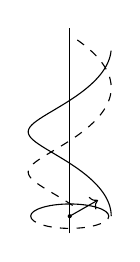
\begin{tikzpicture}[scale=0.62]
                \draw (0,0) -- (0,4.2);
                \draw[dashed] (-0.8,0.35) arc[start angle=180,end angle=360,x radius=0.8,y radius=0.25];
                \draw (-0.8,0.35) arc[start angle=180,end angle=0,x radius=0.8,y radius=0.25];
                \draw[smooth, samples=120, domain=0:6.2]
                    plot ({0.85*cos(\x r)},{0.22*sin(\x r)+0.55*\x+0.35});
                \draw[smooth, dashed, samples=120, domain=0:6.2]
                    plot ({0.85*cos((\x+1.5) r)},{0.22*sin((\x+1.5) r)+0.55*\x+0.35});
                \fill (0,0.35) circle (1.2pt);
                \draw[->] (0,0.35) -- (0.58,0.68);
            \end{tikzpicture}
        \end{minipage}
    \end{wrapfigure}
    Dimostrare che le due eliche circolari
    \[
        \sigma_1(t)=(\cos t,\sin t,at)
    \]
    e
    \[
        \sigma_2(t)=(\cos(t+\theta),\sin(t+\theta),at),
    \]
    con \(\theta\notin 2\pi\mathbb{Z}\), sono contenute nello stesso
    cilindro e non si intersecano.  \wrapfill
\end{snippetexercise}

\begin{snippetsolution}{10 - Doppia elica}
    Consideriamo il caso di una vera elica, cioè \(a\neq 0\). Entrambe le curve sono contenute nel cilindro circolare retto di raggio \(1\) e asse l'asse \(z\), infatti
    \[
        x^2+y^2=\cos^2t+\sin^2t=1
    \]
    per \(\sigma_1\), e analogamente
    \[
        x^2+y^2=\cos^2(t+\theta)+\sin^2(t+\theta)=1
    \]
    per \(\sigma_2\).
    Mostriamo ora che non si intersecano. Supponiamo per assurdo che esistano \(t,s\in\realnumbers\) tali che
    \[
        \sigma_1(t)=\sigma_2(s).
    \]
    Allora, confrontando la terza coordinata, otteniamo
    \[
        at=as.
    \]
    Poiché \(a\neq0\), segue che
    \[
        t=s.
    \]
    Confrontando ora le prime due coordinate, si ha
    \[
        (\cos t,\sin t)=(\cos(t+\theta),\sin(t+\theta)).
    \]
    Questo accade se e solo se
    \[
        \theta\in 2\pi\mathbb{Z},
    \]
    contro l'ipotesi \(\theta\notin2\pi\mathbb{Z}\). Dunque non esistono \(t,s\in\realnumbers\) tali che \(\sigma_1(t)=\sigma_2(s)\), e quindi le due eliche non si intersecano.
    Osserviamo infine che, se \(a=0\), le due curve non sono vere eliche: entrambe parametrizzano la stessa circonferenza \(x^2+y^2=1\), \(z=0\). In quel caso l'enunciato di non intersezione sarebbe falso.
\end{snippetsolution}

\pagebreak

\begin{snippetexercise}{11 - Inviluppo di una famiglia di rette}
    \begin{wrapfigure}{r}{6cm}
        \begin{center}
            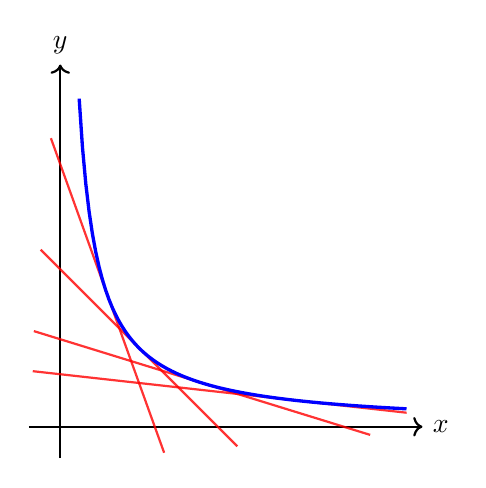
\begin{tikzpicture}[scale=2]
                \draw[->, thick] (-0.2, 0) -- (2.3, 0) node[right] {$x$};
                \draw[->, thick] (0, -0.2) -- (0, 2.3) node[above] {$y$};
                
                \clip (-0.2, -0.2) rectangle (2.2, 2.2);

                \foreach \t in {0.6, 1.0, 1.8, 3.0} {
                    \draw[red, opacity=0.8, thick, shorten >=-10pt, shorten <=-10pt] (0, {1/\t}) -- ({\t}, 0);
                }

                \draw[blue, very thick, domain=0.12:2.2, samples=100] plot (\x, {1/(4*\x)});
            \end{tikzpicture}
            \vspace{-1cm}
        \end{center}
    \end{wrapfigure}
    Calcolare la curva inviluppo della famiglia di rette \(\ell_t\)
    passanti per i punti
    \[
        (t,0)
        \qquad\text{e}\qquad
        \left(0,\frac{1}{t}\right),
        \qquad
        t\in\realnumbers\setminus\{0\}.
    \]
    La retta \(\ell_t\) può essere scritta nella forma
    \[
        F(t,x,y)=0,
        \qquad
        F(t,x,y)=x+t^2y-t.
    \]
    \wrapfill
\end{snippetexercise}

\begin{snippetsolution}{11 - Inviluppo di una famiglia di rette}
    L'inviluppo della famiglia si ottiene risolvendo il sistema
    \[
        \begin{cases}
            F(t,x,y)=0,\\
            F_t(t,x,y)=0.
        \end{cases}
    \]
    Nel nostro caso
    \[
        F(t,x,y)=x+t^2y-t,
    \]
    quindi
    \[
        F_t(t,x,y)=2ty-1.
    \]
    Dobbiamo dunque risolvere
    \[
        \begin{cases}
            x+t^2y-t=0,\\
            2ty-1=0.
        \end{cases}
    \]
    Dalla seconda equazione ricaviamo
    \[
        y=\frac{1}{2t}.
    \]
    Sostituendo nella prima:
    \[
        x+t^2\frac{1}{2t}-t=0,
    \]
    cioè
    \[
        x+\frac{t}{2}-t=0.
    \]
    Quindi
    \[
        x=\frac{t}{2}.
    \]
    L'inviluppo è pertanto parametrizzato da
    \[
        \gamma(t)=\left(\frac{t}{2},\frac{1}{2t}\right),
        \qquad t\in\realnumbers\setminus\{0\}.
    \]
    Eliminando il parametro, da \(t=2x\) otteniamo
    \[
        y=\frac{1}{4x}.
    \]
    Quindi l'equazione cartesiana dell'inviluppo è \(4xy=1\).
\end{snippetsolution}

\pagebreak

\begin{snippetexercise}{12 - Esistenza dell'inviluppo}
    \begin{wrapfigure}{r}{6.25cm}
        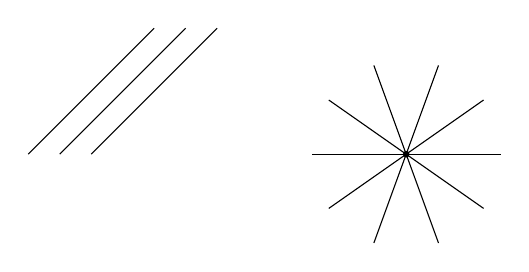
\begin{tikzpicture}[scale=0.8]
            \draw (-2,0)--(0,2);
            \draw (-1.5,0)--(0.5,2);
            \draw (-1,0)--(1,2);

            \begin{scope}[xshift=4cm]
                \foreach \a in {0,35,70,110,145} {
                    \draw (0,0)--({1.5*cos(\a)},{1.5*sin(\a)});
                    \draw (0,0)--({-1.5*cos(\a)},{-1.5*sin(\a)});
                }
                \fill (0,0) circle (1.5pt);
            \end{scope}
        \end{tikzpicture}
        \vspace{-1cm}
    \end{wrapfigure}
    Sia
    \[
        F(t,x,y)=0
    \]
    una famiglia di rette. Dimostrare che la curva inviluppo esiste e
    non è costante se e solo se \(F\) non esprime un fascio di rette. \wrapfill
\end{snippetexercise}

\begin{snippetsolution}{12 - Esistenza dell'inviluppo}
    Scriviamo la famiglia di rette nella forma
    \[
        F(t,x,y)=a(t)x+b(t)y+c(t),
    \]
    con
    \[
        (a(t),b(t))\neq(0,0)
    \]
    per ogni \(t\). L'inviluppo si cerca imponendo il sistema
    \[
        \begin{cases}
            F(t,x,y)=0,\\
            F_t(t,x,y)=0.
        \end{cases}
    \]
    Cioè
    \[
        \begin{cases}
            a(t)x+b(t)y+c(t)=0,\\
            a'(t)x+b'(t)y+c'(t)=0.
        \end{cases}
    \]
    Consideriamo il determinante
    \[
        \Delta(t)=
        \begin{vmatrix}
            a(t) & b(t)\\
            a'(t) & b'(t)
        \end{vmatrix}
        =
        a(t)b'(t)-a'(t)b(t).
    \]
    Se \(\Delta(t)\neq0\), il sistema ha un'unica soluzione, data da
    \[
        x(t)=\frac{b(t)c'(t)-b'(t)c(t)}{\Delta(t)},
        \qquad
        y(t)=\frac{c(t)a'(t)-a(t)c'(t)}{\Delta(t)}.
    \]
    Quindi, sugli intervalli in cui \(\Delta(t)\neq0\), l'inviluppo è la curva
    \[
        \gamma(t)=
        \left(
            \frac{b(t)c'(t)-b'(t)c(t)}{\Delta(t)},
            \frac{c(t)a'(t)-a(t)c'(t)}{\Delta(t)}
        \right).
    \]
    Supponiamo ora che la famiglia sia un fascio proprio, cioè che tutte le rette passino per uno stesso punto \(P_0=(x_0,y_0)\). Allora
    \[
        F(t,x_0,y_0)=0
    \]
    per ogni \(t\). Derivando rispetto a \(t\), otteniamo anche
    \[
        F_t(t,x_0,y_0)=0.
    \]
    Quindi il sistema che definisce l'inviluppo ha sempre la soluzione costante \(P_0\). Se la soluzione è unica, l'inviluppo è proprio la curva costante \(\gamma(t)=P_0\). Dunque un fascio proprio non dà un inviluppo non costante.
    Se invece la famiglia è un fascio improprio, cioè è formata da rette parallele, allora la direzione normale \((a(t),b(t))\) è costante a meno di moltiplicazione per uno scalare. In particolare
    \[
        \Delta(t)=0
    \]
    per ogni \(t\). Il sistema
    \[
        F(t,x,y)=F_t(t,x,y)=0
    \]
    non determina allora una curva di punti di contatto nel piano affine. Anche in questo caso non si ottiene un inviluppo non costante.
    Viceversa, supponiamo che la famiglia non sia un fascio di rette. Allora non può accadere che \(\Delta(t)=0\) per ogni \(t\), perché in tal caso tutte le rette avrebbero la stessa direzione e formerebbero un fascio improprio. Quindi esiste un intervallo in cui
    \[
        \Delta(t)\neq0,
    \]
    e su tale intervallo il sistema \(F=F_t=0\) definisce una curva \(\gamma(t)\). Se questa curva fosse costante, diciamo
    \[
        \gamma(t)=P_0,
    \]
    allora \(P_0\) apparterrebbe a tutte le rette della famiglia, perché
    \[
        F(t,\gamma(t))=0.
    \]
    La famiglia sarebbe quindi un fascio proprio, contro l'ipotesi.
    Pertanto, se \(F\) non esprime un fascio di rette, l'inviluppo esiste ed è non costante. Abbiamo così dimostrato che la curva inviluppo esiste ed è non costante se e solo se la famiglia non è un fascio di rette.
\end{snippetsolution}

\begin{snippetexercise}{13 - Proprietà focale delle coniche}
    Data un'ellisse \[
        E = \{ p \in \realnumbers^2 \suchthat d(P, F_1) + d(P, F_2) = 2a \}
    \]
    Dimostrare che gli angoli di incidenza di \(PF_1\) e \(PF_2\)
    con la tangente ad \(E\) in \(P\) sono uguali.
    Un raggio di luce partente da \(F_1\) verso \(P\)
    è riflesso su \(F_2\), se \(E\) è sup. a specchio.
\end{snippetexercise}

\begin{snippetsolution}{13 - Proprietà focale delle coniche}

    \begin{wrapfigure}{r}{6cm}
        \begin{center}
            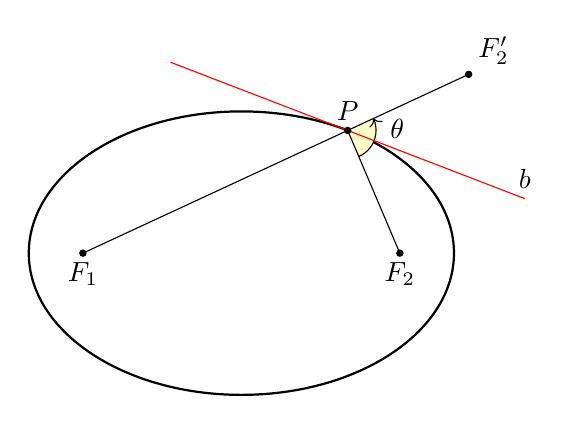
\begin{tikzpicture}[scale=0.9]
                \definecolor{anglecolor}{RGB}{255,255,200}
                
                \draw[thick] (0,0) ellipse (3cm and 2cm);
                
                \coordinate (F1) at (-2.236, 0);
                \coordinate (F2) at (2.236, 0);
                \coordinate (P) at (1.5, 1.732);
                \coordinate (F2p) at (3.207, 2.523);
                \coordinate (T1) at (4, 0.769);
                \coordinate (T2) at (-1, 2.694);
                
                \fill[anglecolor] (P) -- ++(-67:0.4) arc (-67:25:0.4) -- cycle;
                
                \draw[->] ([shift={(-67:0.4)}]P) arc (-67:25:0.4);
                
                \draw (F1) -- (F2p);
                \draw (F2) -- (P);
                
                \draw[red, thin] (T2) -- (T1) node[above, black] {$b$};
                
                \fill (F1) circle (1.5pt) node[below] {$F_1$};
                \fill (F2) circle (1.5pt) node[below] {$F_2$};
                \fill (P) circle (1.5pt) node[above] {$P$};
                \fill (F2p) circle (1.5pt) node[above right] {$F_2'$};
                
                \node at (2.2, 1.75) {$\theta$};
            \end{tikzpicture}
        \end{center}
    \end{wrapfigure}
    Consideriamo al retta \(b\) bisettrice dell'angolo \(\theta\) fra le rette
    \(PF_2\) e \(PF_1\). Vogliamo dimostrare che \(b\) è tangente all'ellisse in \(P\).
    Consideriamo \(F_2'\) su \(PF_1\) con distanza
    \[
        d(P, F_2') = d(P, F_2)
    \]
    dunque
    \[
        d(F_1, F_2') = d(P, F_1) + d(P, F_2)
    \]
    Ogni altro punto \(Q \in b\) con \(Q \neq P\),
    abbiamo \begin{align*}
        d(F_1, Q) + d(F_2, Q)
        &= d(F_1, Q) + d(F_2', Q) \\
        &> d(F_1, F_2') = d(F_1, P) + d(F_2, P)
    \end{align*}
    Notiamo che \(d(Q, F_2) = d(Q, F_2')\) poiché
    \(Q \in b\) che è anche l'asse del segmento \([F_2, F_2']\).
    Quindi ogni \(Q \in b\) con \(Q \neq P\) non può appartenere all'ellisse,
    quindi \(E \intersection b = \{P\}\) e \(b\) deve essere tangente. La tesi segue dalla simmetria
    degli angoli sul vertice.
    \wrapfill
\end{snippetsolution}

\end{document}

\begin{snippetexercise}{14 - Catenaria e trattrice}
    Calcolare l'involuta della catenaria
    \[
        \sigma(x)=(x,\cosh x),
    \]
    partendo dal punto
    \[
        N=(0,1).
    \]
    Ricavare così la parametrizzazione della trattrice
    \[
        \tau(x)=
        \left(
            x-\tanh x,
            \frac{1}{\cosh x}
        \right).
    \]

    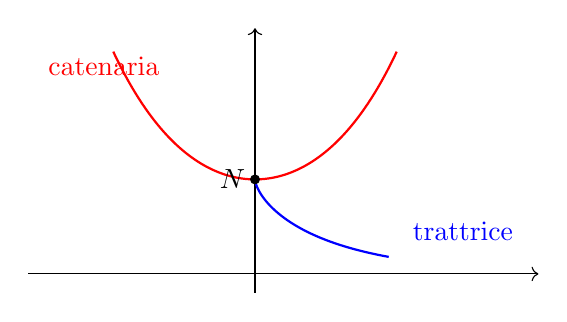
\begin{tikzpicture}[scale=1.2]
        \draw[->] (-2.4,0)--(3,0);
        \draw[->] (0,-0.2)--(0,2.6);

        \draw[red,thick,domain=-1.5:1.5,samples=120,smooth,variable=\u]
        plot ({\u},{0.5*(exp(\u)+exp(-\u))});
        \node[red] at (-1.6,2.2) {catenaria};

        \draw[blue,thick,domain=0:2.4,samples=120,smooth,variable=\u]
        plot
        ({\u-(exp(\u)-exp(-\u))/(exp(\u)+exp(-\u))},{2/(exp(\u)+exp(-\u))});
        \node[blue] at (2.2,0.45) {trattrice};

        \fill (0,1) circle (1.5pt) node[left] {\(N\)};
    \end{tikzpicture}
\end{snippetexercise}

\begin{snippetsolution}{14 - Catenaria e trattrice}
    \todo
\end{snippetsolution}

\begin{snippetexercise}{15 - Giustificazione del nome trattrice}
    Dimostrare che il segmento di tangente da un punto della trattrice
    all'asse \(x\) ha lunghezza costante uguale a \(1\).

    \begin{tikzpicture}[scale=1.15]
        \draw[->] (-0.2,0)--(4,0) node[right] {\(x\)};
        \draw[->] (0,-0.2)--(0,2.2) node[above] {\(y\)};

        \draw[blue,thick,domain=0:3.2,samples=120,smooth,variable=\u]
        plot
        ({\u-(exp(\u)-exp(-\u))/(exp(\u)+exp(-\u))},{2/(exp(\u)+exp(-\u))});

        \coordinate (P) at (1.35,0.55);
        \coordinate (Q) at (2.25,0);

        \fill (P) circle (1.5pt) node[above right] {\(\tau(x)\)};
        \fill (Q) circle (1.5pt) node[below] {\(P(x)\)};
        \draw[red,thick] (P)--(Q);
        \node[red] at (1.85,0.35) {\(1\)};
    \end{tikzpicture}
\end{snippetexercise}

\begin{snippetsolution}{15 - Giustificazione del nome trattrice}
    \todo
\end{snippetsolution}

\begin{snippetexercise}{16 - Proprietà equiangolare della spirale logaritmica}
    Sia
    \[
        \sigma(t)=e^{at}(\cos t,\sin t),
        \qquad
        a>0.
    \]
    Dimostrare che l'angolo tra il vettore \(\overrightarrow{OP}\) e la
    retta tangente a \(\sigma\) nel punto \(P=\sigma(t)\) è costante.

    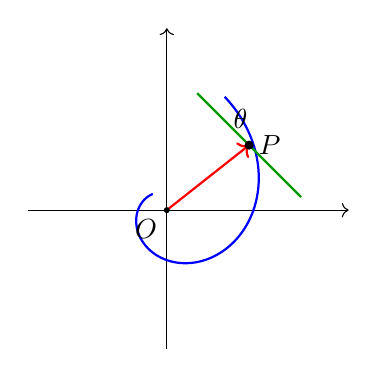
\begin{tikzpicture}[scale=1.1]
        \draw[->] (-1.6,0)--(2.1,0);
        \draw[->] (0,-1.6)--(0,2.1);

        \draw[blue,thick,domain=-4:1.1,samples=180,smooth,variable=\u]
        plot ({exp(0.35*\u)*cos(\u r)},{exp(0.35*\u)*sin(\u r)});

        \coordinate (O) at (0,0);
        \coordinate (P) at (0.95,0.75);
        \draw[red,thick,->] (O)--(P);
        \draw[green!60!black,thick] (0.35,1.35)--(1.55,0.15);

        \fill (O) circle (1pt) node[below left] {\(O\)};
        \fill (P) circle (1.5pt) node[right] {\(P\)};
        \node at (0.85,1.05) {\(\theta\)};
    \end{tikzpicture}
\end{snippetexercise}

\begin{snippetsolution}{16 - Proprietà equiangolare della spirale logaritmica}
    \todo
\end{snippetsolution}

\begin{snippetexercise}{17 - Curvatura e torsione dell'elica circolare}
    Data l'elica circolare
    \[
        \sigma(t)=(\cos t,\sin t,at),
    \]
    calcolare la curvatura \(\kappa_\sigma\) e la torsione \(\tau_\sigma\).
\end{snippetexercise}

\begin{snippetsolution}{17 - Curvatura e torsione dell'elica circolare}
    \todo
\end{snippetsolution}

\begin{snippetexercise}{18 - Caratterizzazione delle eliche circolari}
    Dimostrare che le uniche curve di \(\realnumbers^3\) con
    \[
        \kappa(s)=\text{costante}>0,
        \qquad
        \tau(s)=\text{costante}\neq 0
    \]
    sono eliche circolari del tipo
    \[
        \sigma(t)=(a\cos t,a\sin t,bt),
        \qquad
        a\neq 0,
        \qquad
        b\neq 0.
    \]
\end{snippetexercise}

\begin{snippetsolution}{18 - Caratterizzazione delle eliche circolari}
    \todo
\end{snippetsolution}

\begin{snippetexercise}{19 - Indici di avvolgimento}
    Determinare gli indici di avvolgimento
    \[
        i(\sigma,P)
    \]
    nelle varie componenti connesse di
    \[
        \realnumbers^2\setminus\operatorname{Im}(\sigma),
    \]
    dove \(\sigma\) è la curva regolare disegnata sotto.

    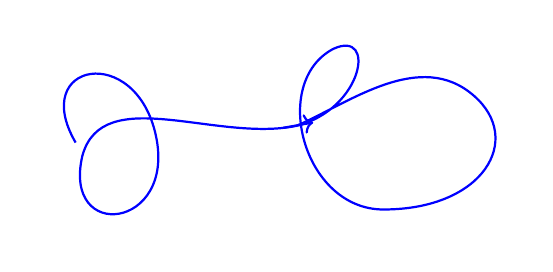
\begin{tikzpicture}[scale=0.85]
        \draw[blue,thick]
        (-3.3,0.2)
        .. controls (-4.0,1.4) and (-2.4,1.7) .. (-2.1,0.3)
        .. controls (-1.8,-1.1) and (-3.5,-1.3) .. (-3.2,0.0)
        .. controls (-2.9,1.1) and (-1.2,0.2) .. (0.0,0.45)
        .. controls (1.0,0.7) and (1.2,1.9) .. (0.55,1.6)
        .. controls (-0.4,1.1) and (0.1,-0.8) .. (1.3,-0.8)
        .. controls (2.8,-0.8) and (3.4,0.25) .. (2.65,0.9)
        .. controls (1.85,1.6) and (0.8,0.8) .. (0.0,0.45);

        \draw[blue,->,thick] (-0.2,0.42)--(0.25,0.5);
    \end{tikzpicture}
\end{snippetexercise}

\begin{snippetsolution}{19 - Indici di avvolgimento}
    \todo
\end{snippetsolution}

\begin{snippetexercise}{20 - Tracce di bicicletta}
    Consideriamo una traiettoria chiusa convessa di una bicicletta di
    lunghezza \(d\), dove \(d\) è la distanza tra i punti di contatto
    delle due ruote con il terreno.

    Dimostrare che l'area racchiusa tra le tracce delle due ruote è
    \[
        \pi d^2.
    \]

    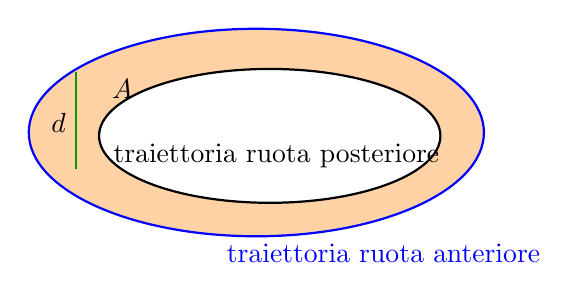
\begin{tikzpicture}[scale=0.85]
        \fill[orange!35,even odd rule]
        (0,0) ellipse (3.4 and 1.55)
        (0.2,-0.05) ellipse (2.55 and 1.0);

        \draw[blue,thick] (0,0) ellipse (3.4 and 1.55);
        \draw[black,thick] (0.2,-0.05) ellipse (2.55 and 1.0);

        \node[blue] at (1.9,-1.8) {traiettoria ruota anteriore};
        \node at (0.3,-0.35) {traiettoria ruota posteriore};
        \node at (-2.0,0.65) {\(A\)};

        \draw[green!60!black,thick] (-2.7,-0.55)--(-2.7,0.9);
        \node[left] at (-2.7,0.15) {\(d\)};
    \end{tikzpicture}

    Vedi suggerimento della Lezione 13.
\end{snippetexercise}

\begin{snippetsolution}{20 - Tracce di bicicletta}
    \todo
\end{snippetsolution}

\begin{snippetexercise}{21 - Spazi proiettivi I}
    Sia \(\mathbb{K}=\realnumbers\) oppure
    \(\mathbb{K}=\complexnumbers\). Dimostrare che la proiezione canonica
    \[
        \pi\colon \mathbb{K}^{m+1}\setminus\{0\}\longrightarrow
        \mathbb{P}^m_{\mathbb{K}},
        \qquad
        v\longmapsto [v],
    \]
    è una mappa \(C^\infty\). Nel caso reale, dimostrare la stessa cosa
    per la restrizione
    \[
        \pi\colon S^m\longrightarrow \mathbb{P}^m_{\realnumbers}.
    \]
    Vedi i suggerimenti della Lezione 15.
\end{snippetexercise}

\begin{snippetsolution}{21 - Spazi proiettivi I}
    \todo
\end{snippetsolution}

\begin{snippetexercise}{22 - Spazi proiettivi II}
    Dimostrare che, per \(m\geq 2\),
    \[
        \pi_1\left(\mathbb{P}^m_{\realnumbers}\right)\neq \{1\}.
    \]
    Più precisamente, si può dimostrare che
    \[
        \pi_1\left(\mathbb{P}^m_{\realnumbers}\right)\simeq \mathbb{Z}_2.
    \]
    Dedurre che
    \[
        \mathbb{P}^m_{\realnumbers}\not\simeq S^m
    \]
    come varietà, per \(m\geq 2\).

    Vedi i suggerimenti della Lezione 15.
\end{snippetexercise}

\begin{snippetsolution}{22 - Spazi proiettivi II}
    \todo
\end{snippetsolution}

\begin{snippetexercise}{23 - Grassmanniane}
    Ricordare la definizione della Grassmanniana
    \[
        G_k(\mathbb{K}^m),
        \qquad
        \mathbb{K}=\realnumbers \text{ oppure } \complexnumbers,
    \]
    cioè dello spazio dei sottospazi vettoriali \(k\)-dimensionali di
    \(\mathbb{K}^m\). Dimostrare, almeno nel caso
    \(\mathbb{K}=\realnumbers\), che
    \[
        G_k(\realnumbers^m)
    \]
    è compatta e di Hausdorff.
\end{snippetexercise}

\begin{snippetsolution}{23 - Grassmanniane}
    \todo
\end{snippetsolution}

\begin{snippetexercise}{24 - Anello di germi di funzioni}
    Sia \(X\) una varietà liscia e sia \(p\in X\). Ricordare la
    definizione dell'anello dei germi di funzioni lisce in \(p\),
    \[
        C^\infty_{X,p}.
    \]
    Dimostrare che \(C^\infty_{X,p}\) è un anello locale e che il suo
    unico ideale massimale è
    \[
        \mathfrak{m}_{X,p}
        =
        \left\{[f]\in C^\infty_{X,p}\mid f(p)=0\right\}.
    \]
\end{snippetexercise}

\begin{snippetsolution}{24 - Anello di germi di funzioni}
    \todo
\end{snippetsolution}

\begin{snippetexercise}{25 - Prodotto di Lie di campi vettoriali}
    Ricordare la definizione del prodotto di Lie di due campi
    vettoriali \(X,Y\), denotato con
    \[
        [X,Y].
    \]
    Dimostrare che \([X,Y]\) è ancora un campo vettoriale. Provare inoltre che
    \[
        [Y,X]=-[X,Y]
    \]
    e che, per ogni funzione derivabile \(f\),
    \[
        [X,fY]=X(f)Y+f[X,Y].
    \]
\end{snippetexercise}

\begin{snippetsolution}{25 - Prodotto di Lie di campi vettoriali}
    \todo
\end{snippetsolution}

\begin{snippetexercise}{26 - Formula di Leibniz-Jacobi per il prodotto di Lie}
    Dimostrare che il prodotto di Lie soddisfa la formula di Jacobi,
    nella forma di Leibniz:
    \[
        [X,[Y,Z]]
        =
        [[X,Y],Z]+[Y,[X,Z]].
    \]
\end{snippetexercise}

\begin{snippetsolution}{26 - Formula di Leibniz-Jacobi per il prodotto di Lie}
    \todo
\end{snippetsolution}

\begin{snippetexercise}{27 - Prodotto vettoriale in \(\realnumbers^3\)}
    Applicare la formula di Jacobi per il prodotto di Lie fra campi
    vettoriali per dimostrare la formula analoga per il prodotto
    vettoriale di \(\realnumbers^3\):
    \[
        u\times(v\times w)
        =
        (u\times v)\times w+v\times(u\times w).
    \]

    Associare a ogni \(v\in\realnumbers^3\) il campo delle velocità di
    rotazione dei punti di \(\realnumbers^3\) attorno all'asse \(v\),
    con velocità angolare \(\|v\|\). Più precisamente, definire
    \(\psi\) sui vettori della base canonica come segue:
    \begin{align*}
        \psi(e_1)
        &=
        -y\frac{\partial}{\partial z}
        +z\frac{\partial}{\partial y},\\
        \psi(e_2)
        &=
        -z\frac{\partial}{\partial x}
        +x\frac{\partial}{\partial z},\\
        \psi(e_3)
        &=
        -x\frac{\partial}{\partial y}
        +y\frac{\partial}{\partial x},
    \end{align*}
    e poi estendere per linearità a tutto \(\realnumbers^3\).

    Provare che
    \[
        \psi(v\times w)=[\psi(v),\psi(w)]
    \]
    e usare la formula di Jacobi del prodotto di Lie per dedurre la
    formula precedente per il prodotto vettoriale.

    \begin{tikzpicture}[scale=0.9]
        \draw[->] (0,0)--(2,0) node[right] {\(x\)};
        \draw[->] (0,0)--(-0.9,-0.8) node[left] {\(y\)};
        \draw[->] (0,0)--(0,2) node[above] {\(z\)};
        \draw[->,thick] (0,0)--(1.2,0.8) node[right] {\(v\)};
        \draw[->] (0.8,0.2) arc (10:100:0.6);
    \end{tikzpicture}
\end{snippetexercise}

\begin{snippetsolution}{27 - Prodotto vettoriale in \(\realnumbers^3\)}
    \todo
\end{snippetsolution}

\begin{snippetexercise}{28 - Spazi tangenti di \(S^m\) e \(\mathbb{P}^m\)}
    Enunciare e dimostrare formule esplicite per gli spazi tangenti
    \[
        T_vS^m
    \]
    e
    \[
        T_{[v]}\mathbb{P}^m_{\realnumbers}.
    \]
    In particolare, per la sfera si deve ottenere
    \[
        T_vS^m=\left\{w\in\realnumbers^{m+1}\mid \langle v,w\rangle=0\right\}.
    \]
    Per lo spazio proiettivo, una descrizione naturale è
    \[
        T_{[v]}\mathbb{P}^m_{\realnumbers}
        \simeq
        \operatorname{Hom}\left(\langle
        v\rangle,\realnumbers^{m+1}/\langle v\rangle\right).
    \]
\end{snippetexercise}

\begin{snippetsolution}{28 - Spazi tangenti di \(S^m\) e \(\mathbb{P}^m\)}
    \todo
\end{snippetsolution}

\begin{snippetexercise}{29 - Embedding di \(\mathbb{P}^2_{\realnumbers}\)
    in \(\realnumbers^4\)}
    Dimostrare che la mappa
    \[
        \phi\colon S^2\longrightarrow \realnumbers^4
    \]
    definita da
    \[
        \phi(x,y,z)=\left(xy,yz,xz,x^2-y^2\right)
    \]
    induce un embedding
    \[
        \iota\colon \mathbb{P}^2_{\realnumbers}\hookrightarrow \realnumbers^4.
    \]
    Usare il diagramma commutativo
    \[
        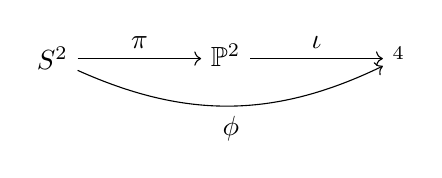
\begin{tikzpicture}[baseline=-0.5ex]
            \node (S) at (0,0) {\(S^2\)};
            \node (P) at (2.2,0) {\(\mathbb{P}^2_{\realnumbers}\)};
            \node (R) at (4.4,0) {\(\realnumbers^4\)};
            \draw[->] (S)--(P) node[midway,above] {\(\pi\)};
            \draw[->] (P)--(R) node[midway,above] {\(\iota\)};
            \draw[->,bend right=25] (S) to node[below] {\(\phi\)} (R);
        \end{tikzpicture}
    \]
    e verificare che \(\phi(v)=\phi(-v)\).
\end{snippetexercise}

\begin{snippetsolution}{29 - Embedding di \(\mathbb{P}^2_{\realnumbers}\)
    in \(\realnumbers^4\)}
    \todo
\end{snippetsolution}

\begin{snippetexercise}{30 - Non orientabilità di \(\mathbb{P}^2_{\realnumbers}\)}
    Dimostrare che il nastro di Möbius non è orientabile e dedurre che
    \[
        \mathbb{P}^2_{\realnumbers}
    \]
    non è orientabile.
\end{snippetexercise}

\begin{snippetsolution}{30 - Non orientabilità di \(\mathbb{P}^2_{\realnumbers}\)}
    \todo
\end{snippetsolution}

\begin{snippetexercise}{31 - Mappa antipodale e riflessione rispetto a un
    piano equatoriale}
    Sia
    \[
        A\colon S^m\longrightarrow S^m,
        \qquad
        A(x)=-x
    \]
    la mappa antipodale.

    \begin{enumerate}
        \item Dimostrare che \(A\) preserva l'orientazione se e solo se
            \(m\) è dispari.
        \item Dimostrare che la riflessione rispetto a un piano equatoriale,
            \[
                R(x_1,\ldots,x_{m+1})
                =
                (-x_1,x_2,\ldots,x_{m+1}),
            \]
            inverte sempre l'orientazione.
    \end{enumerate}
\end{snippetexercise}

\begin{snippetsolution}{31 - Mappa antipodale e riflessione rispetto a un
    piano equatoriale}
    \todo
\end{snippetsolution}

\begin{snippetexercise}{32 - Quali spazi proiettivi reali sono orientabili?}
    Dimostrare che
    \[
        \mathbb{P}^m_{\realnumbers}
    \]
    è orientabile se e solo se \(m\) è dispari.

    Suggerimento: usare il risultato dell'esercizio precedente e la mappa
    \[
        \pi\colon S^m\longrightarrow \mathbb{P}^m_{\realnumbers}
    \]
    per definire un'orientazione di \(\mathbb{P}^m_{\realnumbers}\).
\end{snippetexercise}

\begin{snippetsolution}{32 - Quali spazi proiettivi reali sono orientabili?}
    \todo
\end{snippetsolution}

\begin{snippetexercise}{33 - Differenziale esterno delle \(k\)-forme}
    Dare la definizione di
    \[
        d\omega
    \]
    per \(\omega\) una \(k\)-forma differenziale su \(X\). Dimostrare che
    \[
        d(d\omega)=0.
    \]
    Vedi Lezione 22. Usare la Proposizione 10, se necessario.
\end{snippetexercise}

\begin{snippetsolution}{33 - Differenziale esterno delle \(k\)-forme}
    \todo
\end{snippetsolution}

\begin{snippetexercise}{34 - Metrica della sfera}
    Calcolare la matrice della metrica della sfera di raggio \(R\),
    \[
        S^2_R=\left\{x\in\realnumbers^3\mid \|x\|=R\right\},
    \]
    in coordinate polari. Usando la parametrizzazione
    \[
        \Phi(\theta,\varphi)
        =
        \left(
            R\sin\theta\cos\varphi,
            R\sin\theta\sin\varphi,
            R\cos\theta
        \right),
    \]
    si deve ottenere
    \[
        g
        =
        \begin{pmatrix}
            R^2 & 0\\
            0 & R^2\sin^2\theta
        \end{pmatrix}.
    \]
\end{snippetexercise}

\begin{snippetsolution}{34 - Metrica della sfera}
    \todo
\end{snippetsolution}

\begin{snippetexercise}{35 - Cilindri di carta}
    Dimostrare che esiste un'isometria locale fra un aperto di
    \(\realnumbers^2\) e un cilindro circolare retto.

    Per esempio, per il cilindro di raggio \(R\), considerare
    \[
        \Phi(u,v)=
        \left(
            R\cos\frac{u}{R},
            R\sin\frac{u}{R},
            v
        \right).
    \]
\end{snippetexercise}

\begin{snippetsolution}{35 - Cilindri di carta}
    \todo
\end{snippetsolution}

\begin{snippetexercise}{36 - Coni di carta}
    Sia \(X\) il cono circolare retto definito come grafico di
    \[
        z=\sqrt{x^2+y^2}.
    \]
    Dimostrare che esiste un'isometria locale fra
    \[
        \Omega=\realnumbers^2\setminus\left\{(x,0)\mid x\geq 0\right\}
    \]
    e \(X\).

    Suggerimento: trovare la matrice della metrica euclidea di
    \(\realnumbers^2\setminus\{0\}\) rispetto alle coordinate polari
    \((r,\theta)\), tali che
    \[
        (x,y)=(r\cos\theta,r\sin\theta).
    \]
    Usare le stesse coordinate polari per parametrizzare il cono. In
    particolare, osservare che
    \[
        \Phi(r,\theta)
        =
        \left(
            \frac{r}{\sqrt{2}}\cos(\sqrt{2}\theta),
            \frac{r}{\sqrt{2}}\sin(\sqrt{2}\theta),
            \frac{r}{\sqrt{2}}
        \right)
    \]
    è una parametrizzazione locale di \(X\). Mostrare che la matrice
    della metrica rispetto a \((r,\theta)\) coincide con quella
    euclidea in coordinate polari.

    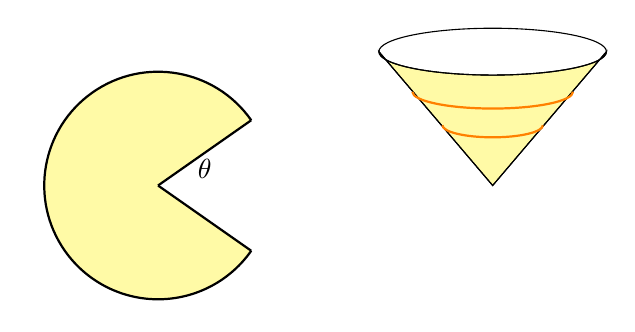
\begin{tikzpicture}[scale=0.85]
        \fill[yellow!35] (0,0) -- (35:1.7) arc (35:325:1.7) -- cycle;
        \draw[thick] (0,0)--(35:1.7);
        \draw[thick] (0,0)--(325:1.7);
        \draw[thick] (35:1.7) arc (35:325:1.7);
        \node at (0.7,0.25) {\(\theta\)};

        \begin{scope}[xshift=5cm]
            \draw[fill=yellow!35] (0,0) -- (-1.7,2) arc (180:360:1.7 and
            0.35) -- cycle;
            \draw (-1.7,2)--(0,0)--(1.7,2);
            \draw (0,2) ellipse (1.7 and 0.35);
            \draw[orange,thick] (-1.2,1.4) arc (180:360:1.2 and 0.25);
            \draw[orange,thick] (-0.75,0.9) arc (180:360:0.75 and 0.18);
        \end{scope}
    \end{tikzpicture}
\end{snippetexercise}

\begin{snippetsolution}{36 - Coni di carta}
    \todo
\end{snippetsolution}

\begin{snippetexercise}{37 - Elicoide}
    Scrivere la matrice della metrica dell'elicoide \(X\) parametrizzato da
    \[
        \psi(x,y)=
        \left(
            y\cos x,
            y\sin x,
            ax
        \right).
    \]
    Si deve ottenere una matrice diagonale:
    \[
        g_X
        =
        \begin{pmatrix}
            y^2+a^2 & 0\\
            0 & 1
        \end{pmatrix}.
    \]
\end{snippetexercise}

\begin{snippetsolution}{37 - Elicoide}
    \todo
\end{snippetsolution}

\begin{snippetexercise}{38 - Catenoide}
    Scrivere la matrice della metrica del catenoide \(Y\) parametrizzato da
    \[
        \varphi(x,y)
        =
        a\left(
            \cosh x\cos y,
            \cosh x\sin y,
            x
        \right).
    \]
    Si deve ottenere
    \[
        g_Y
        =
        a^2\cosh^2 x
        \begin{pmatrix}
            1 & 0\\
            0 & 1
        \end{pmatrix}.
    \]
\end{snippetexercise}

\begin{snippetsolution}{38 - Catenoide}
    \todo
\end{snippetsolution}

\begin{snippetexercise}{39 - Isometria locale elicoide-catenoide}
    Costruire un'isometria locale
    \[
        h\colon X\longrightarrow Y
    \]
    fra l'elicoide e il catenoide degli esercizi precedenti.

    Suggerimento: riparametrizzare l'elicoide nella forma
    \[
        X(u,v)=
        \left(
            a\sinh u\cos v,
            a\sinh u\sin v,
            av
        \right),
    \]
    e il catenoide nella forma
    \[
        Y(u,v)=
        a\left(
            \cosh u\cos v,
            \cosh u\sin v,
            u
        \right).
    \]
    In queste coordinate le due metriche coincidono:
    \[
        g_X=g_Y=a^2\cosh^2 u
        \begin{pmatrix}
            1 & 0\\
            0 & 1
        \end{pmatrix}.
    \]
\end{snippetexercise}

\begin{snippetsolution}{39 - Isometria locale elicoide-catenoide}
    \todo
\end{snippetsolution}

\begin{snippetexercise}{40 - Superfici di rotazione}
    Determinare una parametrizzazione
    \[
        \Psi(t,\theta)
    \]
    della superficie \(S\subseteq\realnumbers^3\) ottenuta ruotando
    attorno all'asse \(z\) la curva
    \[
        \sigma(t)=\left(0,g(t),f(t)\right),
        \qquad
        g(t)>0.
    \]
    La parametrizzazione naturale è
    \[
        \Psi(t,\theta)
        =
        \left(
            g(t)\cos\theta,
            g(t)\sin\theta,
            f(t)
        \right).
    \]
    Scrivere la matrice della metrica di \(S\) rispetto a
    \((t,\theta)\). Cosa succede se la curva \(\sigma\) è
    parametrizzata per lunghezza d'arco?

    In generale:
    \[
        g
        =
        \begin{pmatrix}
            f'(t)^2+g'(t)^2 & 0\\
            0 & g(t)^2
        \end{pmatrix}.
    \]
    Se \(\sigma\) è parametrizzata per lunghezza d'arco, allora
    \[
        f'(t)^2+g'(t)^2=1.
    \]
\end{snippetexercise}

\begin{snippetsolution}{40 - Superfici di rotazione}
    \todo
\end{snippetsolution}

\begin{snippetexercise}{41 - Proiezione stereografica}
    Ricordare la definizione di mappa conforme e dimostrare che la
    proiezione stereografica
    \[
        \pi_N\colon S^2\setminus\{(0,0,1)\}\longrightarrow \realnumbers^2,
    \]
    o equivalentemente la sua inversa, è una mappa conforme.

    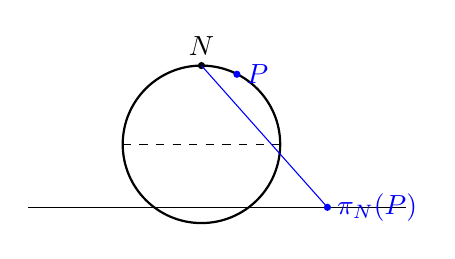
\begin{tikzpicture}[scale=1]
        \draw (-2.2,-0.8)--(2.6,-0.8);
        \draw[thick] (0,0) circle (1);
        \draw[dashed] (-1,0)--(1,0);
        \fill (0,1) circle (1.3pt) node[above] {\(N\)};
        \coordinate (P) at (0.45,0.89);
        \coordinate (Q) at (1.6,-0.8);
        \fill[blue] (P) circle (1.3pt) node[right] {\(P\)};
        \fill[blue] (Q) circle (1.3pt) node[right] {\(\pi_N(P)\)};
        \draw[blue] (0,1)--(Q);
    \end{tikzpicture}
\end{snippetexercise}

\begin{snippetsolution}{41 - Proiezione stereografica}
    \todo
\end{snippetsolution}

\begin{snippetexercise}{42 - Proiezione cilindrica}
    Sia \(S^2\) la sfera di raggio \(1\) e sia \(X\) il cilindro
    circolare retto di raggio \(1\). Definiamo
    \[
        \pi\colon S^2\setminus\{\text{poli}\}\longrightarrow X
    \]
    ponendo \(\pi(P)\) uguale all'intersezione fra \(X\) e la retta
    passante per \(P\) e perpendicolare all'asse \(z\).

    Dimostrare che \(\pi\) preserva le aree.

    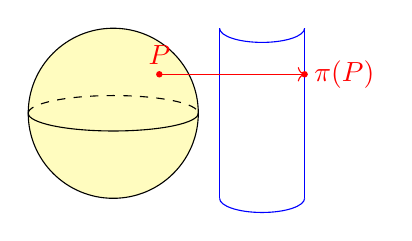
\begin{tikzpicture}[scale=0.9]
        \draw[fill=yellow!25] (0,0) circle (1.2);
        \draw (-1.2,0) arc (180:360:1.2 and 0.25);
        \draw[dashed] (-1.2,0) arc (180:0:1.2 and 0.25);
        \draw[blue] (1.5,-1.2)--(1.5,1.2);
        \draw[blue] (2.7,-1.2)--(2.7,1.2);
        \draw[blue] (1.5,1.2) arc (180:360:0.6 and 0.2);
        \draw[blue] (1.5,-1.2) arc (180:360:0.6 and 0.2);

        \coordinate (P) at (0.65,0.55);
        \coordinate (Q) at (2.7,0.55);
        \fill[red] (P) circle (1.3pt) node[above] {\(P\)};
        \fill[red] (Q) circle (1.3pt) node[right] {\(\pi(P)\)};
        \draw[red,->] (P)--(Q);
    \end{tikzpicture}
\end{snippetexercise}

\begin{snippetsolution}{42 - Proiezione cilindrica}
    \todo
\end{snippetsolution}

\begin{snippetexercise}{43 - Geodetiche della sfera}
    Dimostrare che le geodetiche della sfera
    \(S^2\subseteq\realnumbers^3\) sono tutti e soli gli archi di
    circonferenze massime, cioè di circonferenze con centro coincidente
    con quello della sfera, parametrizzati a velocità scalare costante.
\end{snippetexercise}

\begin{snippetsolution}{43 - Geodetiche della sfera}
    \todo
\end{snippetsolution}

\begin{snippetexercise}{44 - Geodetiche di un cilindro circolare retto}
    Dimostrare che le geodetiche di un cilindro circolare retto
    \[
        X=\left\{(x,y,z)\in\realnumbers^3\mid x^2+y^2=R^2\right\}
    \]
    sono tutte e sole le curve dei seguenti tipi, parametrizzate a
    velocità scalare costante:
    \[
        \text{rette verticali,}
        \qquad
        \text{circonferenze orizzontali,}
        \qquad
        \text{eliche circolari.}
    \]

    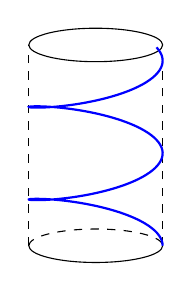
\begin{tikzpicture}[scale=0.85]
        \draw[dashed] (-1,0)--(-1,3);
        \draw[dashed] (1,0)--(1,3);
        \draw (0,3) ellipse (1 and 0.25);
        \draw (-1,0) arc (180:360:1 and 0.25);
        \draw[dashed] (-1,0) arc (180:0:1 and 0.25);

        \draw[blue,thick,domain=0:13,samples=160,smooth,variable=\u]
        plot ({cos(\u r)},{0.22*\u+0.25*sin(\u r)});
    \end{tikzpicture}
\end{snippetexercise}

\begin{snippetsolution}{44 - Geodetiche di un cilindro circolare retto}
    \todo
\end{snippetsolution}

\begin{snippetexercise}{45 - Superfici contenenti rette}
    Dimostrare che, se una superficie \(S\subseteq\realnumbers^3\)
    contiene una retta \(\ell\) o un suo segmento, allora tale retta,
    parametrizzata linearmente, è sempre una geodetica di \(S\).
\end{snippetexercise}

\begin{snippetsolution}{45 - Superfici contenenti rette}
    \todo
\end{snippetsolution}

\begin{snippetexercise}{46 - Geodetiche di un cono}
    Considerare il cono circolare retto a una falda
    \[
        X=
        \left\{
            (x,y,z)\in\realnumbers^3
            \mid
            z=\sqrt{x^2+y^2}
        \right\},
    \]
    già studiato nel problema sui ``coni di carta''.

    Descrivere le coppie di punti \(P,Q\in X\) tali che la curva di
    lunghezza minima che collega \(P\) a \(Q\) sia l'unione dei segmenti
    \[
        [P,O]\union[O,Q],
    \]
    dove \(O=(0,0,0)\) è il vertice del cono.

    Mostrare inoltre che una circonferenza orizzontale su \(X\) non è
    mai una geodetica. Descrivere una parametrizzazione di una
    geodetica arbitraria di \(X\) e mostrare che non può mai essere
    definita su tutto \(\realnumbers\).

    Suggerimento: usare il problema sui coni di carta.
\end{snippetexercise}

\begin{snippetsolution}{46 - Geodetiche di un cono}
    \todo
\end{snippetsolution}

\begin{snippetexercise}{47 - Disco di Poincaré e semipiano superiore di Siegel I}
    Dimostrare che il disco di Poincaré
    \[
        \mathbb{D}
        =
        \{z\in\complexnumbers\mid |z|<1\},
        \qquad
        ds^2_{\mathbb{D}}
        =
        \frac{|dz|^2}{(1-|z|^2)^2},
    \]
    e il semipiano superiore di Siegel
    \[
        \mathbb{H}
        =
        \{z\in\complexnumbers\mid \operatorname{Im}z>0\},
        \qquad
        ds^2_{\mathbb{H}}
        =
        \frac{|dz|^2}{(\operatorname{Im}z)^2},
    \]
    sono conformi ad aperti di \(\realnumbers^2\). In particolare, gli
    angoli fra vettori tangenti in un punto sono gli stessi angoli
    misurati nella metrica euclidea di \(\realnumbers^2\).
\end{snippetexercise}

\begin{snippetsolution}{47 - Disco di Poincaré e semipiano superiore di Siegel I}
    \todo
\end{snippetsolution}

\begin{snippetexercise}{48 - Disco di Poincaré e semipiano superiore di Siegel II}
    Mostrare che la mappa
    \[
        \varphi(z)=i\frac{1-z}{1+z},
        \qquad
        \varphi\colon\mathbb{D}\longrightarrow\mathbb{H},
    \]
    è un'isometria e calcolarne l'inversa. Si ottiene
    \[
        \varphi^{-1}(w)=\frac{i-w}{i+w}.
    \]
\end{snippetexercise}

\begin{snippetsolution}{48 - Disco di Poincaré e semipiano superiore di Siegel II}
    \todo
\end{snippetsolution}

\begin{snippetexercise}{49 - Trasformazioni di Möbius I}
    Dimostrare che le trasformazioni di Möbius
    \[
        f(z)=\frac{az+b}{cz+d},
        \qquad
        a,b,c,d\in\complexnumbers,
        \qquad
        ad-bc\neq 0,
    \]
    formano un gruppo rispetto alla composizione. Dimostrare inoltre
    che mandano circonferenze in circonferenze, intendendo fra le
    circonferenze anche le circonferenze degeneri, cioè le rette.
\end{snippetexercise}

\begin{snippetsolution}{49 - Trasformazioni di Möbius I}
    \todo
\end{snippetsolution}

\begin{snippetexercise}{50 - Trasformazioni di Möbius II}
    Mostrare che ogni trasformazione di Möbius
    \[
        f(z)=\frac{az+b}{cz+d},
        \qquad
        ad-bc\neq 0,
    \]
    definita su
    \[
        \complexnumbers\setminus\left\{-\frac{d}{c}\right\}
    \]
    quando \(c\neq 0\), può essere estesa in modo unico a una mappa
    \[
        \psi\colon \mathbb{P}^1_{\complexnumbers}\longrightarrow
        \mathbb{P}^1_{\complexnumbers}
    \]
    definita da
    \[
        \psi([z_0:z_1])
        =
        [az_0+bz_1:cz_0+dz_1].
    \]
    Denotando con
    \[
        \iota\colon\complexnumbers\longrightarrow
        \mathbb{P}^1_{\complexnumbers},
        \qquad
        \iota(z)=[z:1],
    \]
    si ha
    \[
        f=\iota^{-1}\circ\psi\circ\iota
    \]
    sul dominio di \(f\).

    Il gruppo delle \(\psi\) come sopra, con \(ad-bc\neq 0\), è detto
    \[
        \operatorname{PGL}(2,\complexnumbers),
    \]
    ed è il gruppo degli automorfismi di
    \(\mathbb{P}^1_{\complexnumbers}\) indotti dalle trasformazioni
    lineari invertibili di \(\complexnumbers^2\).
\end{snippetexercise}

\begin{snippetsolution}{50 - Trasformazioni di Möbius II}
    \todo
\end{snippetsolution}

\begin{snippetexercise}{51 (facoltativo) - Trasformazioni di Möbius III: birapporto}
    \begin{enumerate}
        \item Mostrare che, per ogni terna di punti distinti
            \[
                P,Q,R\in\mathbb{P}^1_{\complexnumbers},
            \]
            esiste un'unica trasformazione
            \[
                \psi\in\operatorname{PGL}(2,\complexnumbers)
            \]
            tale che
            \[
                \psi(P)=0=[0:1],
                \qquad
                \psi(Q)=\infty=[1:0],
                \qquad
                \psi(R)=1=[1:1].
            \]

            Provare che, se \(P=a\), \(Q=b\), \(R=c\) sono punti di
            \(\complexnumbers\), allora la restrizione a
            \(\complexnumbers\) dell'unica trasformazione \(\psi\) tale che
            \[
                \psi(a)=0,
                \qquad
                \psi(b)=\infty,
                \qquad
                \psi(c)=1
            \]
            è la trasformazione di Möbius
            \[
                f(z)
                =
                \frac{z-a}{z-b}\frac{c-b}{c-a}.
            \]

        \item Definire il birapporto di quattro punti distinti
            \(a,b,d,c\in\complexnumbers\) ponendo
            \[
                \operatorname{Bir}(a,b;d,c)
                =
                \frac{a-d}{b-d}\frac{b-c}{a-c}.
            \]
            La definizione si estende anche al caso in cui uno dei punti
            sia \(\infty\), usando le formule limite corrispondenti.

        \item Dimostrare che il birapporto è invariante per
            trasformazioni di Möbius.
    \end{enumerate}

    Suggerimento: usare il punto precedente per osservare che
    \[
        \operatorname{Bir}(a,b;d,c)=f(d),
    \]
    dove \(f\) è l'unica trasformazione di Möbius tale che
    \[
        f(a)=0,
        \qquad
        f(b)=\infty,
        \qquad
        f(c)=1.
    \]
    Dedurre da questo l'invarianza.
\end{snippetexercise}

\begin{snippetsolution}{51 (facoltativo) - Trasformazioni di Möbius III: birapporto}
    \todo
\end{snippetsolution}

\begin{snippetexercise}{52 - Isometrie di \(\mathbb{H}\)}
    Dimostrare che il sottogruppo delle trasformazioni di Möbius
    \[
        \operatorname{PSL}(2,\realnumbers)
        =
        \left\{
            z\longmapsto \frac{az+b}{cz+d}
            \ \middle|\
            a,b,c,d\in\realnumbers,\ ad-bc=1
        \right\}
    \]
    agisce come gruppo di isometrie su \(\mathbb{H}\).
\end{snippetexercise}

\begin{snippetsolution}{52 - Isometrie di \(\mathbb{H}\)}
    \todo
\end{snippetsolution}

\begin{snippetexercise}{53 - Transitività di
    \(\operatorname{PSL}(2,\realnumbers)\) su \(\mathbb{H}\)}
    Dimostrare che l'azione di \(\operatorname{PSL}(2,\realnumbers)\)
    su \(\mathbb{H}\) è transitiva. Equivalentemente, dati
    \[
        z_1,z_2\in\mathbb{H},
    \]
    esiste
    \[
        g\in\operatorname{PSL}(2,\realnumbers)
    \]
    tale che
    \[
        g(z_1)=z_2.
    \]

    Procedere con i seguenti passi.

    \begin{enumerate}
        \item Dimostrare che le omotetie
            \[
                z\longmapsto kz,
                \qquad
                k>0,
            \]
            stanno in \(\operatorname{PSL}(2,\realnumbers)\). Dedurre che
            \(\operatorname{PSL}(2,\realnumbers)\) agisce transitivamente
            sui numeri puramente immaginari
            \[
                ai,
                \qquad
                a>0.
            \]

        \item Dimostrare che ogni circonferenza con centro in
            \[
                \partial\mathbb{H}=\realnumbers
            \]
            può essere mandata sull'asse immaginario.

        \item Dimostrare che per ogni coppia di punti di \(\mathbb{H}\)
            esiste una circonferenza come sopra che li contiene. Concludere
            usando i punti precedenti.
    \end{enumerate}

    Vedi dimostrazione del Teorema 6, Lezione 31.
\end{snippetexercise}

\begin{snippetsolution}{53 - Transitività di
    \(\operatorname{PSL}(2,\realnumbers)\) su \(\mathbb{H}\)}
    \todo
\end{snippetsolution}

\begin{snippetexercise}{54 - Geodetiche di \(\mathbb{H}\) e di \(\mathbb{D}\)}
    Mostrare che le geodetiche di \(\mathbb{H}\) sono gli archi di
    circonferenze perpendicolari al bordo
    \[
        \partial\mathbb{H}=\realnumbers,
    \]
    incluse le rette verticali, viste come circonferenze passanti per
    \(\infty\).

    Mostrare analogamente che le geodetiche di \(\mathbb{D}\) sono gli
    archi di circonferenze perpendicolari al bordo
    \[
        \partial\mathbb{D}=\{z\in\complexnumbers\mid |z|=1\},
    \]
    inclusi i diametri.

    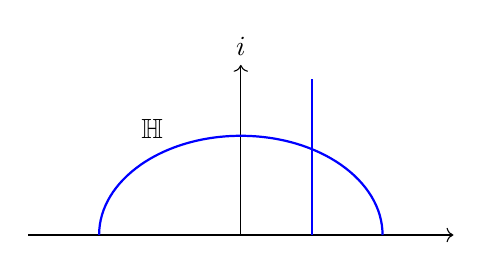
\begin{tikzpicture}[scale=0.9]
        \draw[->] (-3,0)--(3,0) node[right] {\(\realnumbers\)};
        \draw[->] (0,0)--(0,2.4) node[above] {\(i\realnumbers\)};
        \draw[blue,thick] (-2,0) arc (180:0:2 and 1.4);
        \draw[blue,thick] (1,0)--(1,2.2);
        \node at (-1.25,1.5) {\(\mathbb{H}\)};
    \end{tikzpicture}
\end{snippetexercise}

\begin{snippetsolution}{54 - Geodetiche di \(\mathbb{H}\) e di \(\mathbb{D}\)}
    \todo
\end{snippetsolution}

\begin{snippetexercise}{55 (facoltativo) - Formula della distanza di due punti in \(\mathbb{H}\)}
    Dimostrare la seguente formula per la distanza fra due punti
    \[
        z_1,z_2\in\mathbb{H}:
    \]
    \[
        d(z_1,z_2)
        =
        \operatorname{arcosh}
        \left(
            2\operatorname{Bir}(z_1,z_2;\overline{z_2},\overline{z_1})-1
        \right),
    \]
    dove \(\operatorname{arcosh}\) è la funzione inversa di \(\cosh\),
    definita su \([1,+\infty)\).

    Suggerimento: considerare prima il caso in cui i punti siano
    sull'asse immaginario. Nel caso generale, usare una trasformazione
    di Möbius reale che mandi la circonferenza geodetica passante per
    \(z_1,z_2\) sull'asse immaginario e poi applicare l'invarianza
    del birapporto.

    \begin{tikzpicture}[scale=0.9]
        \draw[->] (-3,0)--(3,0);
        \draw[->] (0,0)--(0,2.6);
        \draw[blue,thick] (-2,0) arc (180:0:2 and 1.4);
        \fill (-2,0) circle (1.2pt) node[below] {\(a\)};
        \fill (2,0) circle (1.2pt) node[below] {\(b\)};
        \fill (-0.7,1.3) circle (1.2pt) node[above] {\(z_1\)};
        \fill (0.8,1.3) circle (1.2pt) node[above] {\(z_2\)};
    \end{tikzpicture}
\end{snippetexercise}

\begin{snippetsolution}{55 (facoltativo) - Formula della distanza di due punti in \(\mathbb{H}\)}
    \todo
\end{snippetsolution}

\begin{snippetexercise}{56 - Somma degli angoli interni di un triangolo
    nel piano iperbolico}
    Mostrare che la somma degli angoli interni di un triangolo a lati
    geodetici di \(\mathbb{H}\) può assumere ogni valore
    \[
        0<S<\pi.
    \]
\end{snippetexercise}

\begin{snippetsolution}{56 - Somma degli angoli interni di un triangolo
    nel piano iperbolico}
    \todo
\end{snippetsolution}

\begin{snippetexercise}{57 - Somma degli angoli interni di un triangolo in
    geometria sferica}
    Mostrare che la somma degli angoli interni di un triangolo a lati
    geodetici su una sfera può assumere ogni valore
    \[
        \pi<S<5\pi.
    \]
\end{snippetexercise}

\begin{snippetsolution}{57 - Somma degli angoli interni di un triangolo in
    geometria sferica}
    \todo
\end{snippetsolution}

\end{document}
